\chapter{Tests and Results}

\paragraph{}
A general approach to evaluating question answer tasks is using the mean reciprocal rank (MRR). The score for an individual question is the reciprocal of the rank at which the first correct answer is returned or 0 if no correct response is returned. The score for the run is then the mean over the set of questions in the test. The number of questions for which no correct response is returned is also reported. We use. a similar approach for our evaluation of the question answer systems in Yioop. The Question Answer System implemented is part of the Yioop search engine and is platform independent. The system works by tagging phrases using a Brill variant Part of Speech tagger for Hindi sentences. In the next step, triplets are formed and stored in the database using the grammar rules for Hindi. The test data for the system is an index created by configuring Yioop to crawl Hindi webpages from Wikipedia and Indian websites with Hindi content. We describe the experiments conducted on the Question Answer Module as a standalone utility and next we describe the results when integrated in Yioop.

\section {Question Answer Module: Standalone Testcase}
In this section, we describe test cases for the system as standalone module. It is assumed that the input to the system is a processed to remove special characters, punctuations, etc. Also, the given sentence is semantically and syntactically correct.

\paragraph{}
Figure~\ref{fig:sentence_testcase1} shows the sentence after it is tagged for parts of speech

\begin{figure}[htb]
\centering
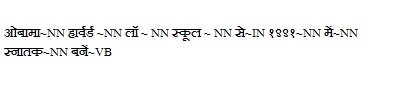
\includegraphics[width=0.8\textwidth]{images/sentence_testcase1.jpg}
\caption{Hindi Sentence 1.} 
\label{fig:sentence_testcase1}
\end{figure}

A word for word translation of the above sentence to English is 'Obama Harvard law school from 1999 graduate complete'. Figure~\ref{fig:standalone_testcase} shows the Parse Tree generated for this sentence 

\begin{figure}[htb]
\centering
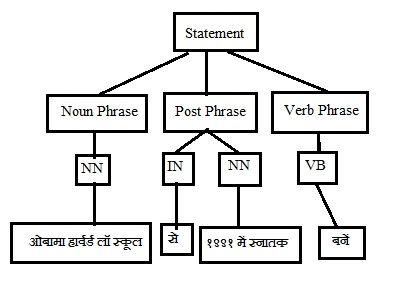
\includegraphics[width=0.8\textwidth]{images/standalone_testcase.jpg}
\caption{Parse Tree for sentence in Figure 7.} 
\label{fig:standalone_testcase}
\end{figure}

\paragraph{}
The triplets extracted for the above parse tree are as shown in Figure~\ref{fig:triplet_standalone}.

\begin{figure}[htb]
\centering
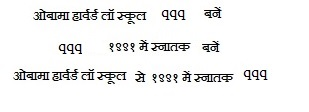
\includegraphics[width=0.8\textwidth]{images/triplet_standalone.jpg}
\caption{Triplets Extracted for sentence Figure 8.} 
\label{fig:triplet_standalone}
\end{figure}

\break
\paragraph{}
Figure~\ref{fig:sentence_testcase2} shows the sentence after it is tagged for parts of speech

\begin{figure}[htb]
\centering
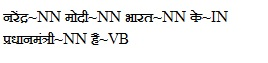
\includegraphics[width=0.5\textwidth]{images/sentence_testcase2.jpg}
\caption{Hindi Sentence 2.} 
\label{fig:sentence_testcase2}
\end{figure}

A word for word translation of the above sentence to English is 'Narendra Modi India (s) Prime Minister is'. Figure~\ref{fig:standalone_testcase2} shows the Parse Tree generated for this sentence 

\begin{figure}[htb]
\centering
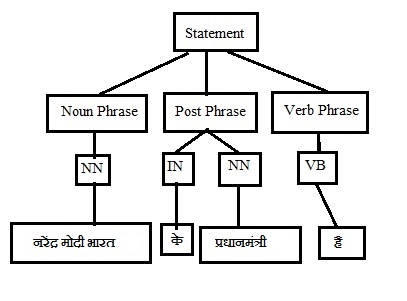
\includegraphics[width=0.8\textwidth]{images/standalone_testcase2.jpg}
\caption{Parse Tree for sentence in Figure 10.} 
\label{fig:standalone_testcase2}
\end{figure}

\break
\section{Question Answer Module Integrated in Yioop}
\paragraph{}
Below are results for the Question Answer System when a crawl was setup for all wikipedia pages in Hindi, Indian websites. We set up a crawl by configuring Yioop in under crawl options. For the crawl, we restrict the crawler to websites from domains \textit{hi.wikipedia.org}, \textit{co.in} and \textit{in}. We stopped the crawl  after we hit 200,000 urls. The crawler extracted information from 7925 webpages to create the index. Figure~\ref{fig:QA_IntegratedInYioop},  Figure~\ref{fig:Yioop_NoQA}, show the results after the Question Answer system is integrated in Yioop. 

\begin{figure}[htb]
\centering
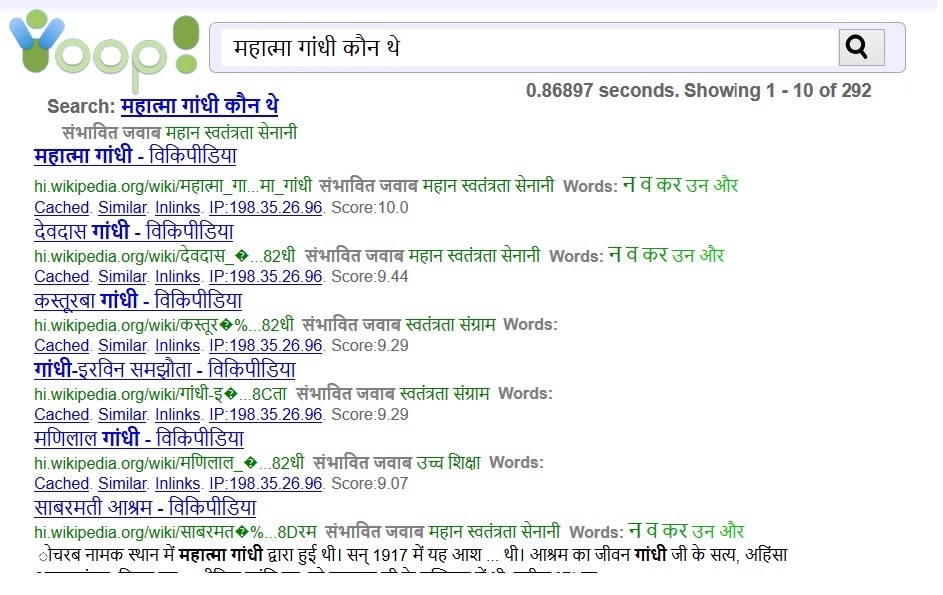
\includegraphics[width=0.9\textwidth]{images/QA_IntegratedInYioop.jpg}
\caption{Question Answer Integration in Yioop.} 
\label{fig:QA_IntegratedInYioop}
\end{figure}
\break

\begin{figure}[htb]
\centering
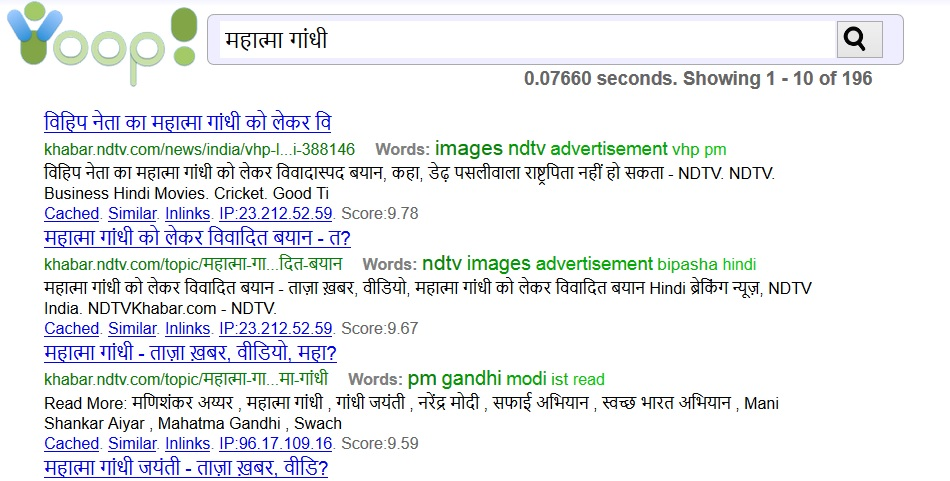
\includegraphics[width=0.8\textwidth]{images/Yioop_NoQA.jpg}
\caption{No Question Answer System in Yioop.} 
\label{fig:Yioop_NoQA}
\end{figure}

\paragraph{}
The integration of the Question Answer system slows down Yioop as extra processing is performed while generating and storing the triplets. But the performance improves for query time as whenever the  user enters a question it is looked up directly from a map. Figure~\ref{fig:QA_performance1} shows the time impact when we asked a simple question in Hindi.

\begin{figure}[htb]
\centering
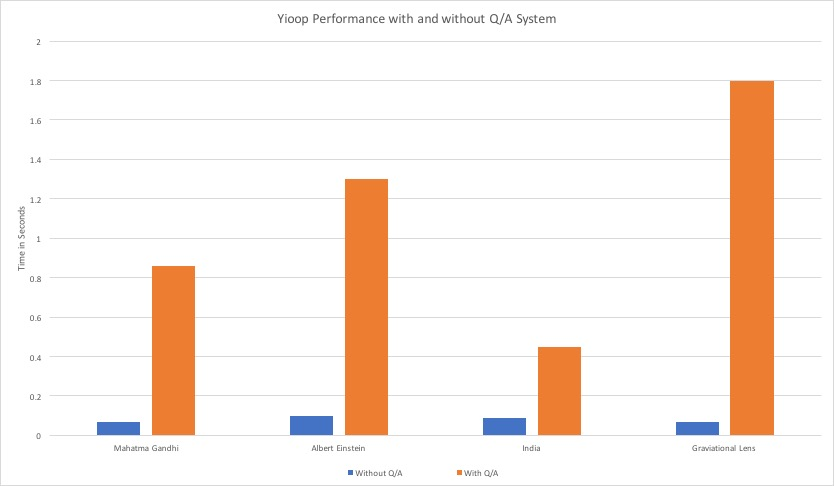
\includegraphics[width=0.8\textwidth]{images/Yioopwith_withoutQA_Hindi.jpg}
\caption{Yioop performance before and after integration of Q/A System.} 
\label{fig:QA_performance1}
\end{figure}

\paragraph{}
The initial implementation of the Question Answer system read performed part of speech tagging by reading a file based lexicon from a file. It performed a sequential search on the lexicon read in memory, Figure~\ref{fig:QA_performance2} shows the improvement in part of speech tagging, as words are tagged from the database indexed on term and locale. For the test, I used 1000 - 1500 word paragraphs for each of the subjects as input to the two variants of the part of speech tagger module.

\begin{figure}[htb]
\centering
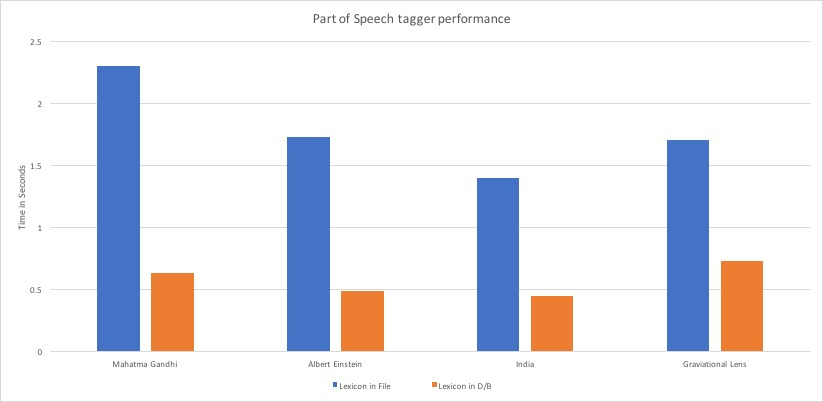
\includegraphics[width=0.8\textwidth]{images/YioopPoS_performance.jpg}
\caption{Part of Speech tagging time comparison.} 
\label{fig:QA_performance2}
\end{figure}
\break

\paragraph{}
We compare the English and Hindi Question answer systems for relevant answers. I used 4 topics on which I asked the same set of questions in English and Hindi. Figure~\ref{fig:QA_performance3} shows the number of correct answers retrieved on Page 1 of the search result. We can see that English system is better at providing more accurate answers compared to Hindi. 

\begin{figure}[htb]
\centering
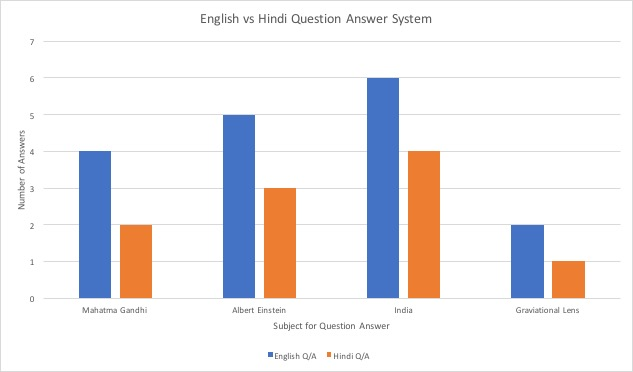
\includegraphics[width=0.8\textwidth]{images/QA_performance3.jpg}
\caption{English v/s Hindi Question Answer System.} 
\label{fig:QA_performance3}
\end{figure}

\break
\paragraph{}
We calculate the mean reciprocal rank for the same set of questions asked to the English and Hindi Question Answer systems. Figure~\ref{fig:score_table} shows the reciprocal ranks for Hindi

\begin{figure}[htb]
\centering
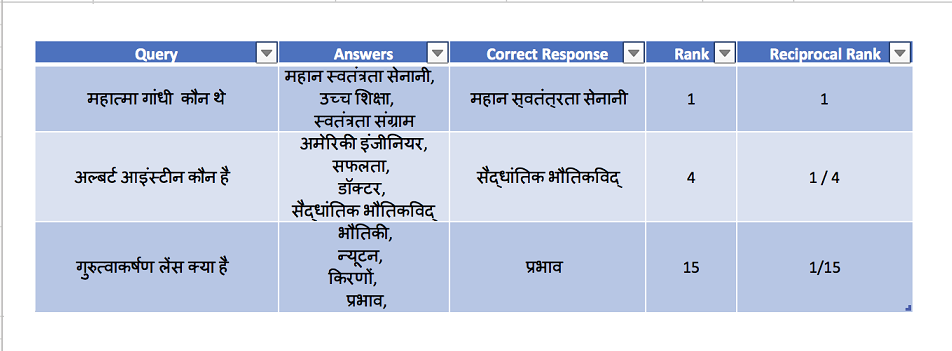
\includegraphics[width=0.8\textwidth]{images/score_table.jpg}
\caption{Reciprocal Rank for Hindi Question Answers.} 
\label{fig:score_table}
\end{figure}

\paragraph{}
We compare the English and Hindi Question Answer System on the  Average Precision scores. Average  Precision is basically the number of correct answers interpreted as correct from the total number of results returned. Figure~\ref{fig:AveragePrecisionScore} shows the score comparison between the 2 systems.

\begin{figure}[htb]
\centering
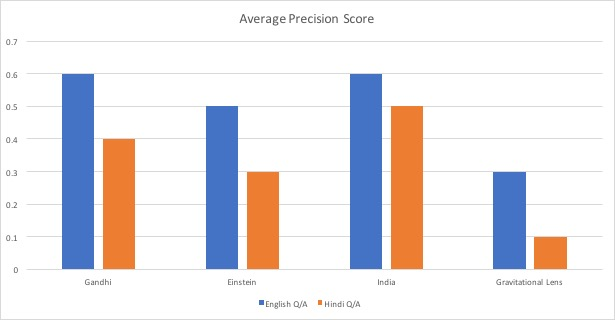
\includegraphics[width=0.8\textwidth]{images/AveragePrecisionScore.jpg}
\caption{Average Precision Score.} 
\label{fig:AveragePrecisionScore}
\end{figure}

\paragraph{}
The Mean Average Precision (MAP), as the name says is the mean of all the average precision scores is the measure of accuracy of a information retrieval system. For our test with the Question Answer sytem integration in Yioop,  I observed the MAP to be 0.43 for Hindi Question Answer system and 0.61 for the English Question Answer System.

\paragraph{}
The systems are tested for accuracy comparing the answers retrieved against a known set of answers. I used a set of 25 questions with a corresponding set of answers which are known to be true. I then asked the same questions to the English and Hindi question answering systems in Yioop. Figure~\ref{fig:Accuracy_EnglishQA} and Figure~\ref{fig:Accuracy_HindiQA} show the efficiency of the systems for simple questions.

\begin{figure}[htb]
\centering
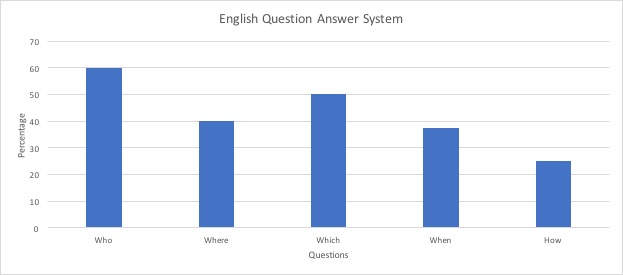
\includegraphics[width=0.8\textwidth]{images/Accuracy_EnglishQA.jpg}
\caption{Accuracy of English Q/A in Yioop.} 
\label{fig:Accuracy_EnglishQA}
\end{figure}

\begin{figure}[htb]
\centering
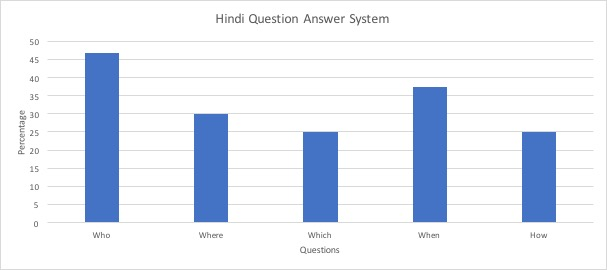
\includegraphics[width=0.8\textwidth]{images/Accuracy_HindiQA.jpg}
\caption{Accuracy of Hindi Q/A in Yioop.} 
\label{fig:Accuracy_HindiQA}
\end{figure}
